\documentclass[twocolumn]{article}
\usepackage{upquote}
\usepackage{listings}
\usepackage{color}
\usepackage[margin=1cm]{geometry}
 \usepackage{graphicx}
%\usepackage{wrapfig}
\begin{document}

\title{Autonomous Trading Agent Implementation Using Natural Language Processing Of News Headlines: An Introduction}
\author{William Lyon}
\date{\today}
\maketitle

\abstract{Natural Language Processing techniques are used to examine financial news headlines and generate predictions of stock price movements.  

\section{Introduction}
\subsection{Motivation}
This tool could be used as a component of an autonomous trading agent that will make BUY/SELL decisions for tradin financial instruments.
\subsection{Literature Review}

\section{Data}
Google Finance provides access to historical stock quotes as well as links to financial news stories pertaining to specific stocks. This data provides the basis for this paper.
\begin{figure}[htb]
%\begin{wrapfigure}{o}{8cm}
\centering
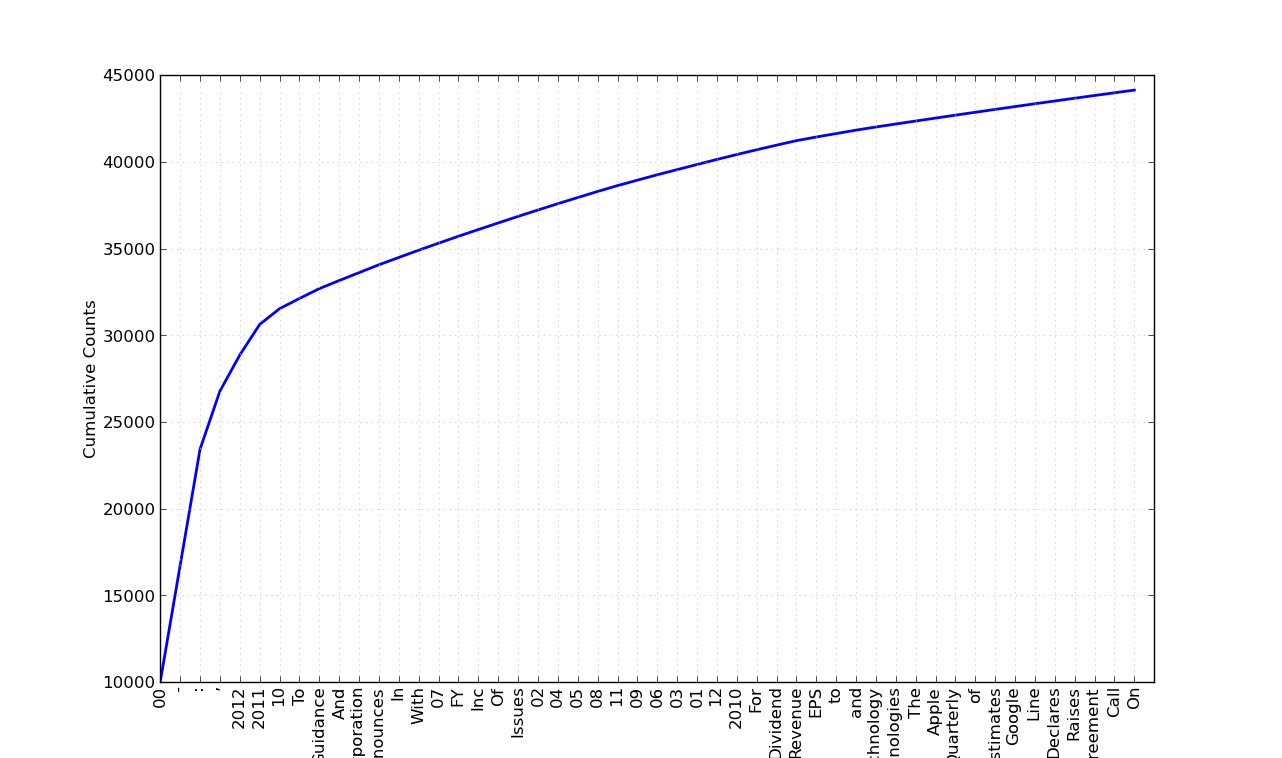
\includegraphics[scale=0.25]{cum_graph.png}
\caption{Cumulative frequency plot}
\end{figure}
%\end{wrapfigure}
%\end{figure}
%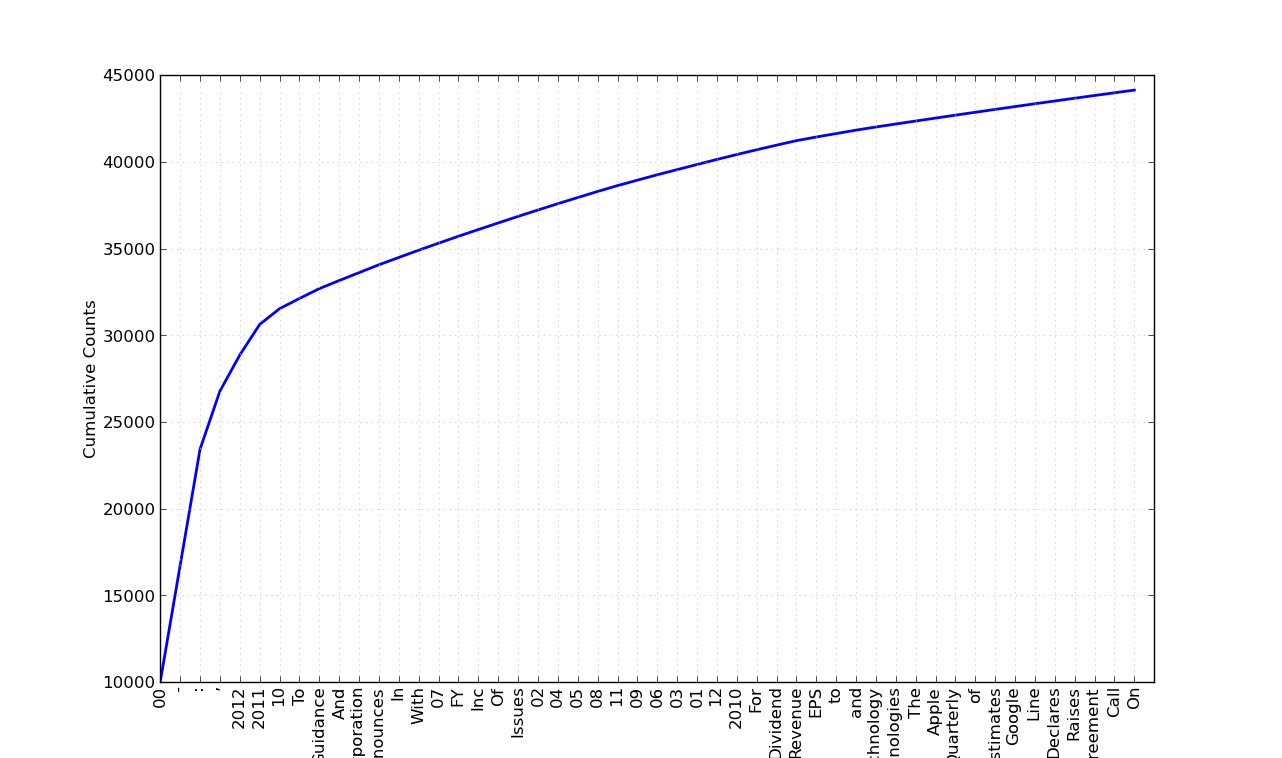
\includegraphics[width=60mm]{cum_graph.png}
%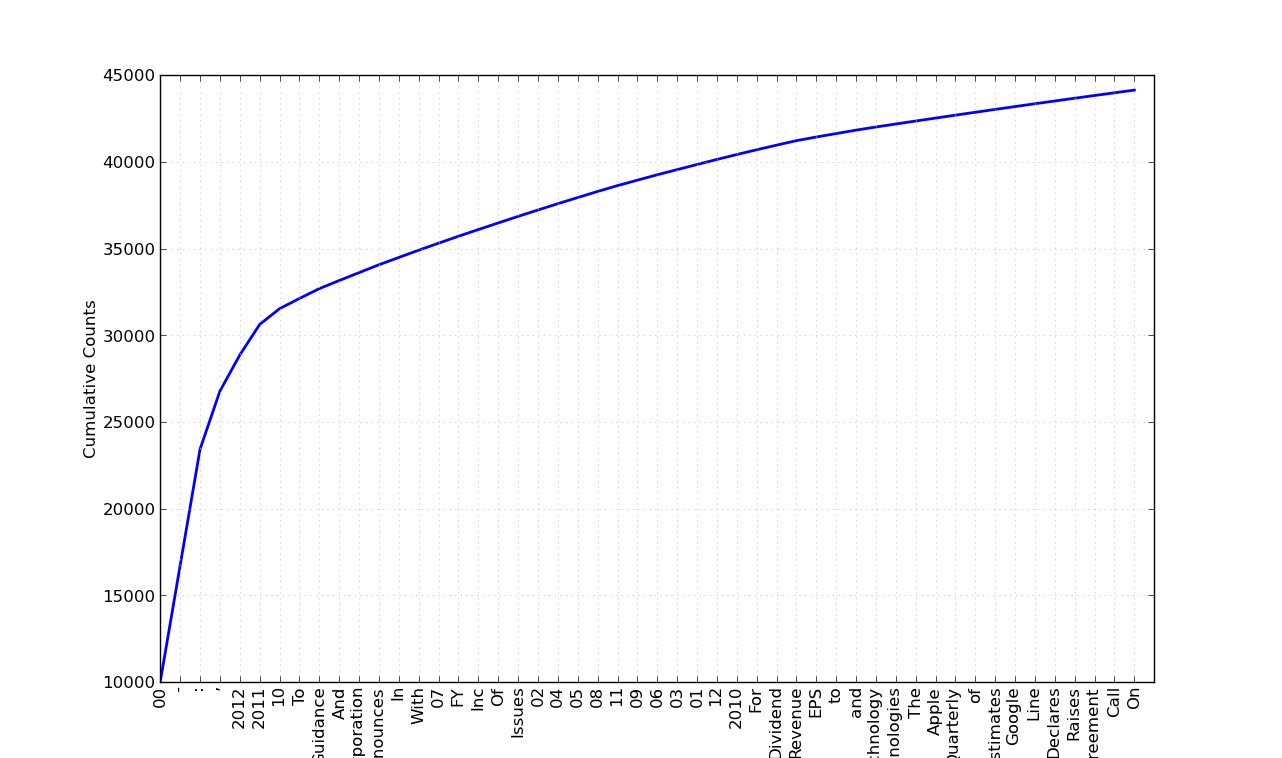
\includegraphics[height=60mm]{cum_graph.jpg}
%\includegraphics[scale=0.75]{myfig.pdf}
%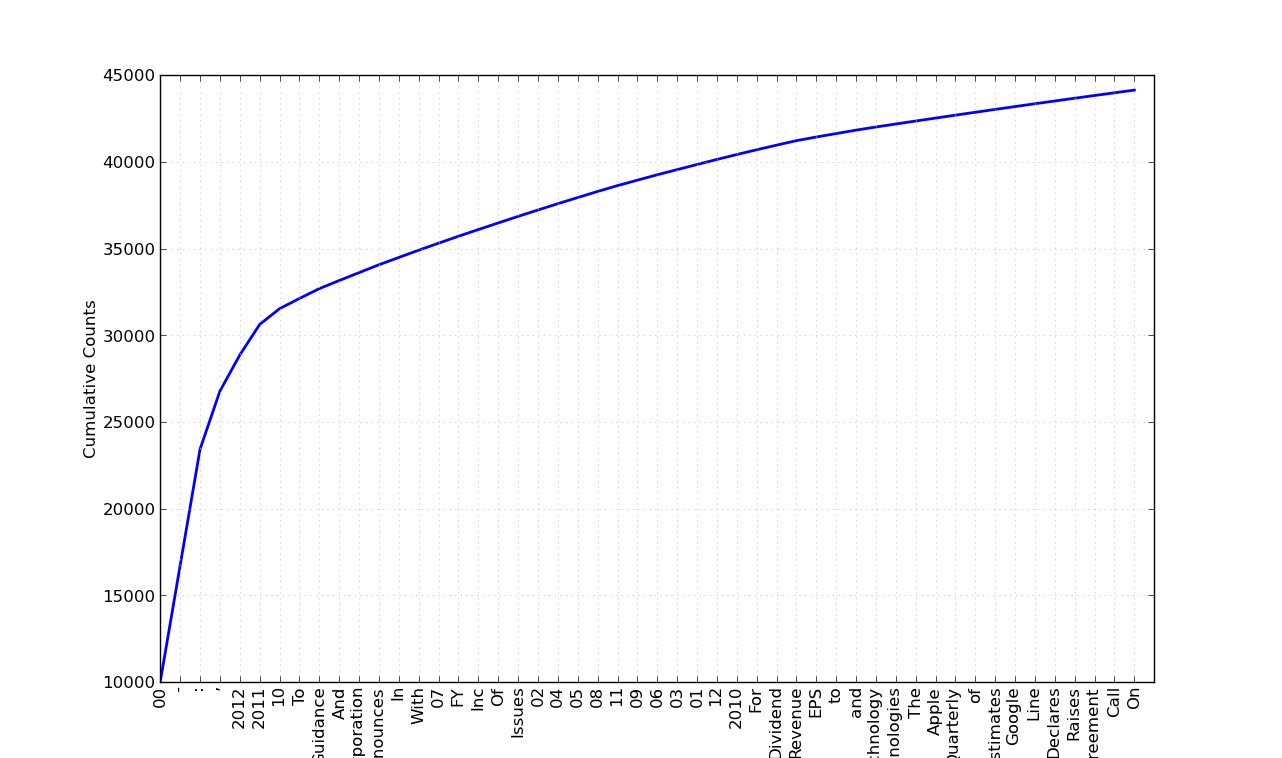
\includegraphics[angle=45,width=52mm]{cum_graph.png}


\section{Methodology}
\subsection{Naive Bayes}

\subsection{Decision Tree}

\subsection{Maximum Entropy}

\section{Implementation}

\section{Evaluation}
\subsection{Accuracy}

\subsection{Most informative features}

\subsection{Precision}

\subsection{Recall}

\section{Conclusions}
\subsection{Further research}

\section{References}
\end{document}